\section{Authentication process}

\begin{itemize}
    \item \href{https://syfuhs.net/how-authentication-works-when-you-use-remote-desktop}{How authentication works when you use remote desktop}
    \item \href{https://techcommunity.microsoft.com/t5/security-compliance-and-identity/azure-advanced-threat-protection-credssp-exploit-analysis/ba-p/250556}{Azure Advanced Threat Protection: CredSSP Exploit}
    \item \href{https://learn.microsoft.com/en-us/previous-versions/windows/it-pro/windows-10/security/threat-protection/security-policy-settings/network-security-allow-pku2u-authentication-requests-to-this-computer-to-use-online-identities}{Network security: Allow PKU2U authentication requests to this computer to use online identities}
    \item \href{https://awakecoding.com/posts/rdp-nla-with-azure-ad-the-pku2u-nightmare/}{RDP NLA with Azure AD: The PKU2U Nightmare}
    \item \href{https://cyber.gouv.fr/sites/default/files/IMG/pdf/Securite_de_RDP_article.pdf}{Sécurité de RDP}
    \item \href{https://www.sstic.org/media/SSTIC2020/SSTIC-actes/analyse_de_la_scurit_rdp__nla_quel_apport_pour_vot/SSTIC2020-Slides-analyse_de_la_scurit_rdp__nla_quel_apport_pour_votre_scurit_-bertoli_bourguenolle.pdf}{Sécurité RDP : Intecteption
    d’authentification sur NLA avec
    CredSSPy}
\end{itemize}

\subsection{Process}

The first thing the client does is ask what protocol is supported. In this case the target responded and said please do NLA~\ref{windows:nla} The client then immediately prompts for credentials. Doesn't do anything special, just prompts.

Once the user enters their creds NLA kicks in. NLA is the first stage of the CredSSP protocol, which is how those creds you typed in make it to the target server securely. NLA works by first opening an SPNEGO~\ref{windows:spnego} Negotiate connection with the target.

The target happily responds and depending on a few conditions might do a couple different things:
\begin{itemize}
    \item first case [\href{https://www.thehacker.recipes/ad/movement/kerberos#user-to-user-authentication}{U2U}]: the target provides its machine account's Kerberos TGT. The client does a TGS-REQ asking for a TGS  to the target name \verb+termsrv/target.domain.com+, and passes the TGT into the \verb+additional-tickets+ field to do something called user-to-user or encrypt-in-session-key authentication
    \item second case: he client just requests a ticket to \verb+termsrv/target.domain.com+ the usual way
    \item third case: NTLM happens
    \item fourth case [PKU2U~\ref{windows:pku2u}]: This is special to AAD-joined target machines only
\end{itemize}

The client converts the ticket into an AP-REQ and fires it off to the target. The target receives it and decrypts it using either the session key in it's machine TGT, or using it's machine password

The target then generates a session key and stashes it in a place LSA can get to. An AP-REP is returned to the client containing this session key

now CredSSP takes those creds and encrypts them using the session key. The client then fires this blob off to the target server.

And the target receives the blob. It takes the session key it stashed away a while back and decrypts the blob. Now it has a username and password. That username and password is passed to the logon UI bits and now we're back to that original thread.

There are some notable differences here though. For instance remote connections never go through cached logon.


\subsection{Network Level Authent:ication (NLA)}
\label{windows:nla}

Network Level Authentication (NLA) is a feature of Remote Desktop Services (RDP Server) or Remote Desktop Connection (RDP Client) that requires the connecting user to authenticate themselves before a session is established with the server.

Originally, if a user opened an RDP (remote desktop) session to a server it would load the login screen from the server for the user. This would use up resources on the server, and was a potential area for denial of service attacks as well as remote code execution attacks (see BlueKeep). Network Level Authentication delegates the user's credentials from the client through a client-side Security Support Provider and prompts the user to authenticate before establishing a session on the server.


\subsection{Remote credential guard}
See~\ref{windows:remote_credential_guard}

\begin{figure}[!ht]
    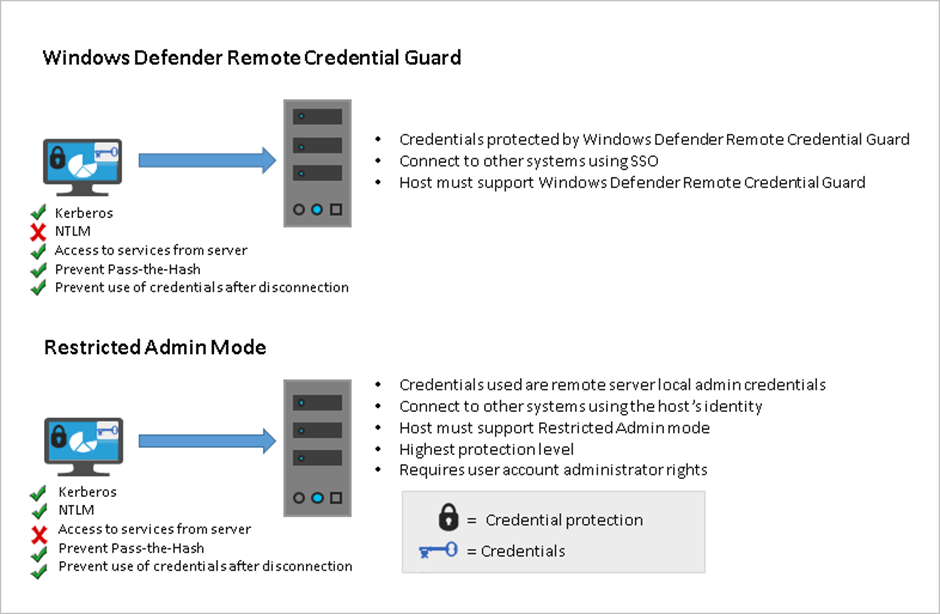
\includegraphics[width=\linewidth]{network/rdp/images/restrictedadmin-rcg.png}
    \caption{restrictedadmin-rcg}
    \label{fig:restrictedadmin-rcg}
\end{figure}

\subsection{Restricted admin}
See~\ref{windows:retricted_admin}